\chapter{Model realization\label{chap:modelReal}}


%Detailed enough to be able to reproduce
%Pseudocode where applicable
%Explain along figure?
%Include technology that's used
%How did we realize/achieve the ideas?
%Present what kind of assumptions/prior knowledge is made!!

%\begin{itemize}
%	\item Actual architectures resemble concepts closely
%	\item Crux lies in the regression model (AITM)
%\end{itemize}
The previous chapter introduced two concepts that were develop with the goal of adapting themselves to unknown situations through interaction.
In order to evaluate the developed ideas, prototypes of the two concepts have been implemented in Python 2.7. Both prototypes are developed as such that they can be evaluated in the same way in the next chapter. The implementations follow the presented concepts very closely in most cases. As such the general data flow is the same as was presented in the figures  \ref{fig:PairPrediction}, \ref{fig:PairPlanning}, \ref{fig:GatePrediction} and \ref{fig:GatePlanning}.
Relevant implementation details as well as made assumptions are highlighted and explained in this chapter.

Section \ref{sec:basics} starts with describing common design decisions that apply to both concepts. Afterwards the relevant implementations details regarding the two prototypes are presented in section \ref{sec:pairRealization} for the interaction state concept and in section \ref{sec:gateRealization} for the object state concept. Finally, section \ref{sec:technologies} describes the used technologies, the underlying regression and classification model and the implementation of the inverse model, in detail.

\section{Basics \label{sec:basics}}

\subsection{Available information about objects}

The kind of information that is provided by the environment obviously depends on the sensors that are available to the robot. From the information provided by these sensors, features can be computed. The models themselves are greatly independent of what features are actually used. In fact the models do not require any knowledge about what the features represent for prediction. This allows the exact same model to be used in various settings with different features, for example if additional or different sensors are available. In order to yield good results, the used features obviously need to have the necessary expressiveness.

Unfortunately, the models do need to have some partial knowledge about the features when it comes to computing action primitives as will be further explained in the corresponding sections for both models.

These prototypes were evaluated using a physics simulation, further explained in section \ref{sec:environment}. From this simulation the information in table \ref{tab:availInformation} is provided for each object at each update.

\begin{table}[h!]
	\centering
	\begin{tabular*}{\textwidth}{@{\extracolsep{\fill} } l l}
		\textbf{Feature} & \textbf{Description} \\ 
		\hline \hline 
		x Position & Global x position of the object \\
		y Position & Global y position of the object \\
		Orientation & Global orientation around the z-axis of the object \\
		x Velocity & Global x velocity of the object \\
		y Velocity & Global y velocity of the object \\
		\hline 
	\end{tabular*} 
	\caption{Summary of all information about objects that is provided by the environment at each update step.}
	\label{tab:availInformation}
\end{table}

Furthermore, a unique identifier, the shape and size of the objects are known and can be used to compute additional features. What kind of features are computed from this information is a design decision by the user of these models. Since the underlying regression model is memory-based, using more features might result in worse performances. This is even more likely, if the features are not normalized or no suitable metric is used.

\subsection{Action primitives}

Action primitives are the collection of possible low level actions a robot can perform directly. Higher level actions are usually composed of multiple action primitives. For example, the action \textit{walking} might be composed of the action primitives \textit{raise leg} and \textit{lower leg}.

In the scope of this thesis, the action primitives are defined by the simulation used for the evaluations in the next chapter. In this case a two dimensional action primitive is used, representing the $x$ and $y$ velocity of the actuator. The velocities are given according to the global coordinate system of the robot. 
In general, the nature of the action is not all that important to the models as long as it can be represented as a vector. 
However, the models assume that an action primitive is selected and performed at every iteration. This is also true for the used velocity action primitives, even if the velocity does not change by using the same action primitive again. 

The used simulation only accepts velocities with a norm not higher than $0.5\frac{m}{s}$. The implementations make sure to scale all computed action primitives accordingly. While moving towards a target, the implementations scale the action primitives to a norm of $0.3\frac{m}{s}$ in order to not push the objects too far.

\subsection{Used regression and classification model}

As already stated in the introduction and motivated in chapter \ref{chap:stateOfTheArt}, this thesis uses a memory-based approach to learn the interactions. For this end, a special adaptation of the \gls{gng} has been developed which can be used for regression as well as classification tasks. This adaptation, called \acrfull{aitm} and explained in section \ref{sec:ITM}, is used for all regression and classification models used in both prototypes unless stated otherwise. 

\subsection{Using local features and predicting differences \label{sec:localFeatures}}

Both prototypes only use local (differential) features as inputs for their trained regression and classification models. 
Local features mean that all features are represented relative to some reference object's coordinate frame. The exact computation of the features is explained in sections \ref{sec:intFeatures} for the interaction state model and \ref{sec:gateFeatures} for the gating model.
Using local features assumes that similar interactions behave identical regardless of where they take place in the environment. 
Only the local relations between the involved objects determine the outcome of the interaction. 
For the given task of pushing interactions this assumption will hold true as long as the environment only has constant effects on the objects. The environment used for the evaluations, described in section \ref{sec:environment}, fulfills these conditions since it only affects the objects through gravity and friction, which are constant in the given scenario. 

The great advantage of this approach is that the interactions can be learned regardless of the object's actual configuration in the environment. In fact training data from all configurations can be used to learn a certain interaction. Furthermore, this approach provides free generalization to any configuration in the environment without the need of additional training data.

In more realistic environments, where this assumption does not hold true, the local features can still be used. However, in this case, additional features containing the information about the influence of the environment or the current object configuration might be required. Depending on the actual scenario and its dynamics, this might require absolute global features which offer a lot less generalization.

An additional consequence of these local features is that the forward models of both concepts can only predict the changes instead of resulting features. As already stated in the two concept descriptions, the actual predictions for the interaction state and the object state are computed by adding these predicted changes to the current states.
Without knowledge about the actual position in the input data, the actual position after an interaction cannot be predicted. However, this is not a problem but rather a benefit. Changes are limited in their size compared to the resulting features. 
Consider the feature position: An object cannot change its position from one timestep to another arbitrarily, but rather only by a certain maximum amount. When predicting changes, the learner's output only needs to cover the subspace defined by this maximum amount instead of the entire space. Furthermore, this approach of only predicting the changes can also be applied when using global input features. The models themselves are therefore not restricted by this.


\section{Modeling pairwise interaction \label{sec:pairRealization}}

The implementation of the pairwise interaction model contains the components visualized in the overview figure \ref{fig:PairOverview}.
The \acrfull{acs} trains a classifier that selects any of the $n$ learned \glspl{ac}. Within each \glspl{ac}, there exist a local forward model which performs the predictions.
However, instead of training local inverse models for each \gls{ac}, one global inverse model is used in this implementation. The reasons for this decision are explained in section \ref{sec:pairPlanningReal}.
Just as the local ones would, the global inverse model returns preconditions that result in a specific change of the interaction state.
The forward model as well as the selector both use the same underlying mechanism in the \acrfull{aitm}. For the reasons explained in section \ref{sec:invModel}, the special \acrfull{tiim} is used for the global inverse model.

As mentioned before, the model is constantly updated with new information provided by the environment. The steps that are performed to update the model each time new information is received are explained in algorithm \ref{alg:intUpdate}.

\begin{algorithm}
\begin{algorithmic}[1]
	\Require{New worldstate ws}
	\Require{Used action $act$}
	\Data{Last worldstate ws$_\text{old}$}
	\Data{Set of Abstract Collections L}
	\Data{Inverse Model IM}
	\Data{Abstract Collection Selector ACS}
	\Statex
	\ForAll{interaction state i $\in$ ws}
		\Let{i$_\text{old}$}{extractInteractionState(ws$_\text{old}$, i)}
		\Let{newEpisode}{Episode(i$_\text{old}$, $act$, i)}
		\Let{$S$}{computeChangedFeatures(newEpisode)}
		\If{$S$ $\notin$ L} \Comment{Check if a corresponding AC already known} 
			\Let{newAC}{AbstractCollection($S$)}
			\Let{L}{L $\cup$ newAC}
		\EndIf
		\Let{AC}{L$_S$} \Comment{The Abstract Collection responsible for $S$} 
		\State update AC with newEpisode
		\State update IM with newEpisode
		\State update ACS with i$_\text{old}$, $act$ and AC
	\EndFor
\end{algorithmic}
\caption{Overview of the update steps in the pairwise interaction state model.}
\label{alg:intUpdate}
\end{algorithm}

%\begin{algorithm}
%	\KwIn{New worldstate ws}
%	\KwIn{Used action $act$}
%	\KwData{Last worldstate ws$_\text{old}$}
%	\KwData{Set of Abstract Collections L}
%	\KwData{Inverse Model IM}
%	\KwData{Abstract Collection Selector ACS}
%	\BlankLine
%	\ForEach{interaction state i $\in$ ws}{
%		i$_\text{old}$ = extractInteractionState(ws$_\text{old}$, i)
%		newEpisode = Episode(i$_\text{old}$, $act$, i) \\
%		$S$ = computeChangedFeatures(newEpisode) \\
%		\tcc*[h]{Check if a corresponding AC already known} \\
%		\If{$S$ $\notin$ L}{
%			newAC = AbstractCollection($S$) \\
%			L = L $\cup$ newAC 
%		}
%		AC = L$_S$ \tcc*[f]{The Abstract Collection responsible for $S$} \\
%		update AC with newEpisode \\
%		update IM with newEpisode \\
%		update ACS with i$_\text{old}$, $act$ and AC
%	}
%	\caption{Prediction of the update steps in the pairwise interaction model.}
%	\label{alg:intUpdate}
%\end{algorithm}

The changed feature set $S$ is computed according to equation \ref{eq:difSet}\footnote{Since local features are used, both $Pre$ and $Post$ need to be transformed to the same coordinate frame, see section \ref{sec:episodes} for details.}. The structure and used features within the interaction state are explained in section \ref{sec:intFeatures} while the episodes are explained in section \ref{sec:episodes}.

When updating an \gls{ac} its forward model needs to be updated. The forward model is trained using the combination of the old interaction state  i$_\text{old}$ and the action primitive $act$ as input and the difference vector $\vec{d}$ between the old and the new interaction state as desired output. The exact training of the \gls{aitm} is explained in section \ref{sec:ITM}. 

The global inverse model is trained on the same features as the forward model. Details regarding the training process are explained in section \ref{sec:invModelRealization}.

The \gls{acs} is also trained on the same combination of i$_\text{old}$ and $act$ as input, but it uses the identifier of the responsible \gls{ac} as desired output.
Since the selector also uses the \gls{aitm} as classifier, the exact update rules are explained below.

When used for prediction the model follows the process visualized in figure \ref{fig:PairPrediction} and described in section \ref{sec:pairPrediction}.
Computing suitable action primitives on the other hand is more complicated and requires additional knowledge about the features. While the general process follows what is explained in \ref{sec:pairPlanning}, the process of providing relevant interaction states as targets and extracting relevant action primitives from the returned preconditions is explained in section \ref{sec:pairPlanningReal}.

%The model itself only works on interaction states and action primitives. The specific structure and content of these features is explained in section \ref{sec:intFeatures}.


\subsection{Used features \label{sec:intFeatures}}

The pairwise interaction model basically only uses the interaction state and the action primitive vector as feature vectors. The actual composition of the interaction state depends on the objects that need to be represented. For this thesis, only simple objects (e.g. spheres or rectangular cubes) are present in the scene which allow fairly simple interaction states as described in table \ref{tab:pairInteractionFeatures}.

\begin{table}
	\centering
	\begin{tabular*}{\textwidth}{@{\extracolsep{\fill} } l l}
		\textbf{Feature} & \textbf{Description} \\ 
		\hline \hline 
		 Id 1 & Identifier of the reference object \\ 
		 Id 2 & Identifier of the second object \\ 
		 Local x Position & Local x position of the reference object \\
		 Local y Position & Local y position of the reference object \\
		 Local Orientation & Local orientation of the reference object \\
		 Relative x Position & Relative x position of the second object \\
		 Relative y Position & Relative y position of the second object \\
		 Relative Orientation & Relative orientation of the second object \\
		\hline 
	\end{tabular*} 
	\caption{Features used to represent one interaction state. Relative positions and velocities refer to the coordinate system of the reference object.}
	\label{tab:pairInteractionFeatures}
\end{table}

As already mentioned in section \ref{sec:localFeatures} differential features are used. Apart from the features listed in the table, the interaction state contains the information required for the transformations. Specifically, the matrix $T$ used to transform from the local coordinate frame back to the global frame, its inverse $T^{-1}$ and the orientation of the reference object in the global coordinate frame are stored.

The interaction states are computed as follows:
All features are computed by transforming the global features of both objects given by the environment to the local coordinate frame. Consider two objects $o_1$ and $o_2$ with positions $\vec{p}_1$ and $\vec{p}_2$ and orientations $\alpha_1$ and $\alpha_2$ respectively. First the transformation matrices $T$ and $T^{-1}$ are computed from the reference object's position and orientation:

\begin{equation}
T = \begin{pmatrix}
\cos(\alpha_1) & -\sin(\alpha_1) & p_{x1} \\
\sin(\alpha_1) & \cos(\alpha_1) & p_{y1} \\
0.0 & 0.0 & 1.0
\end{pmatrix}
\qquad
T^{-1} = inv(T)
\label{eq:transMatrix}
\end{equation}

$p_{x1}$ and $p_{y1}$ correspond to the $x$ and $y$ dimensions of the position $\vec{p}_1$. With the help of the transformation matrix $T^{-1}$ it is possible to compute the local positions, e.g.:

\begin{equation}
\vec{p}' = T^{-1} \times \vec{p}_1^*
\end{equation}

where $\vec{p}_1^*$ is the homogeneous vector of $\vec{p}_1$. Since $\vec{p}'$ is also in homogeneous coordinates, only the first two components are used for the interaction state. The local and relative orientations are computed by subtracting the orientation of the reference object from the given orientations. In fact by doing this, all local fields in the interaction state will be zero after the computation. However, these fields are still required. The \glspl{ac} predict the change in the current interaction state. In order to extract the predicted object states from the interaction state, changes in the reference object need to be predicted as well. 

The object states are extracted by using the inverse transformation. Since the structure of the interaction states are known outside of the model, the predicted local position $\vec{q}$ can easily be extracted. Using the homogeneous coordinates $\vec{q}^*$ of $\vec{q}$, the prediction for the actual object's position $\vec{p}_{pred}$ can be computed:

\begin{equation}
\vec{p}_{pred}^* = T \times \vec{q}^*
\end{equation}

Velocities can be computed analogously if needed.
In order to get the global orientation, the reference object's orientation simply needs to be added to the predicted orientation. 

The model assumes, that these interaction states come directly from the environment. Transformations from and to the actual object states need to be performed outside of the actual model. This is achieved by introducing a \textit{Worldstate}. From the point of view of the model, this worldstate is simply a collection of all interaction states in the environment. At each update from the environment, a new worldstate is computed from the provided information. The model predicts a new worldstate by making predictions about all interaction states that are included in a given worldstate. Since one is usually more interested in the actual object states, the model finalizes the worldstate after all interaction states have been predicted. This finalization extracts the object state predictions from the predicted interaction states. 

\subsection{Episodes \label{sec:episodes}}

Episodes are used to store past experiences. The idea comes from case-based-reasoning \cite{cbr} where past experiences are used to reason about new problems. An episode is made up of three parts: 
\begin{enumerate}
\item The initial interaction state $Pre$ that was given before an action was performed.
\item The action that has been performed.
\item The resulting interaction state $Post$.
\end{enumerate}

As explained in the concept, these experiences can be stored and looked up at query time in order to make predictions. However, as highlighted before, the performance of such an operation deteriorates over time as the number of stored experiences increases. Instead, the \glspl{ac} use these episodes as training data for the local regression model. Apart from those three parts, all episodes compute a difference vector between the initial and resulting interaction state. 
However, since the model is working with local coordinates, it is important that both states are transferred to the same coordinate frame before computing the difference. As explained above, the features in all interaction states are always computed relative to the reference object's coordinate frame. As such the positional information of the reference object will always be zero in a freshly computed interaction state. However, this does not mean, that the reference object has not moved within an episode. The model is interested in learning to predict how a given interaction state changes after a special action is performed. Therefore, the difference vector in an episode needs to represent the differences relative to the initial interaction state. This is achieved by first transforming the features of the $Post$ state back to global coordinates via $T_{Post}$ and then transforming them to the local coordinate frame of the $Pre$ state using $T^{-1}_{Pre}$. For the position of the reference object $p_{ref}$ (in homogeneous coordinates) this can be computed as follows:

\begin{equation}
\vec{p}'_{ref} = T^{-1}_{Pre} \times T_{Post} \times \vec{p}_{ref}
\end{equation}

When transforming the orientation of the $Post$ state, first the global orientation of $Post$'s reference object is added before subtracting $Pre$'s global orientation. All transformed features from $Post$ are again collected in a vector $Post^*$ where the features are organized in the same way as in a normal interaction state.

Afterwards the difference vector can simply be computed by:

\begin{equation}
\vec{d} = Post^* - Pre
\end{equation}

During training, the \glspl{ac} extract the feature differences that they are responsible for from $\vec{d}$ and use those as target output of the local regression model.
Finally, the set of changing features $S$ can then again be computed as stated in equation \ref{eq:difSet} while substituting $Post$ with $Post^*$.

\subsection{From target object state to action primitives\label{sec:pairPlanningReal}}

In most cases the robot will have to push a certain object to a given specification. It usually does not matter where the actuator is after the target is reached. Therefore, it would be best if a target object state could be provided instead of a target interaction state. However, the model itself does not know about object states. Therefore, this prototype implements a method to convert a given object state to an interaction state, where only the reference object is correctly set. The actuator is used as secondary object, however the actuator's features are not required. Instead, the features representing the reference object are remembered in order to only focus on these features when trying to reduce the distance to the target interaction state. 

Once a target interaction state has been computed, the current interaction state between the reference object of interest and the actuator can be retrieved. Using the target interaction state as resulting state, an episode with an empty action is computed. The episode provides the local difference vector\footnote{Here local means that the difference vector is computed in the current interaction state's coordinate frame.} between the current situation and the target configuration. Only the features remembered when constructing the target interaction states are considered from this difference vector. Effectively, these features correspond to the local differences in the object states. 

Following the concept provided in section \ref{sec:pairPlanning}, this reduced difference vector would be used to find the \gls{ac} that is responsible for changes represented in the vector.
Having said that, since only changes of a subset of the entire interaction state are considered, there will usually not be an \gls{ac} that is responsible exactly for these changes. 
Instead there will be several \glspl{ac}, that are responsible for changes in these features. In theory, the \gls{ac} responsible for the most feature changes should be chosen in this situation. 

Unfortunately, the developed inverse model does not work well with the segmentation performed by the \glspl{ac}. The main reason for that is, that the inverse model trains separate prototypes for each feature dimension.
Each prototype tries to learn the preconditions that have the most influence on the given feature dimension. However, a single feature dimension is often represented in multiple \glspl{ac}. Therefore, each local inverse model would only experience a subset of the preconditions responsible for changes in a specific feature dimension. When the \gls{tiim} is trained only on these local parts, the prototypes do not learn the preconditions well.

On top of that, the \gls{tiim} is a model with close to constant update and query times\footnote{The number of prototypes and averages that are learned per prototype are independent of the number of training examples. See section \ref{sec:invModelRealization} for details.}. Therefore, the main reasons for training multiple local models do not apply to this inverse model.

It is for these reasons, that this implementation deviates from the concept in this point and only trains a single global inverse model.
This global inverse model is queried just as a local one would be and returns suitable preconditions given a difference vector.

Once preconditions have been retrieved from the inverse model, the current situation is compared to these preconditions. Most importantly, the current actuator position needs to be similar to the actuator position in the preconditions. If the distance between these two positions is too great, the actuator is circled around the object. Unfortunately, this requires some world knowledge about the objects. In the given implementation, the interaction states defined by the user provide the ability to compute an action primitive that lets the actuator circle around the reference object at a fixed distance (see Appendix \ref{sec:circling} for details). 
Using this circling action the actuator is able to move towards the desired position without influencing the object.

Once the distance is below a threshold of 0.1m\footnote{The threshold heavily depends on the given environment and the size of the objects. This threshold has been empirically determined and worked well in the evaluation environment described in section \ref{sec:environment}.}, the model assumes that the actuator is on the correct side of the object and can move directly towards the desired position. This can be done by simply following the direction between the target position and the current position.

As soon as the actuator has come close\footnote{This implementation uses the threshold of 0.01 to determine when it is close enough.} enough to the position defined by the preconditions, the actual desired action primitive can be computed. The preconditions already contain local action primitives that were encountered during training. These can be transformed to the global coordinate frame using the transformation matrix $T$ from the current interaction state as described above. 

In case no preconditions could be retrieved, for example because the inverse model has not seen training examples that produces changes in the required directions, the model would need to explore. Real strategic exploration is not developed in this thesis, which is why this implementation uses a random action primitive in the general direction of the object in this case. This can lead to the model getting stuck which is why for the purpose of this thesis both models assume, that all required changes have been experienced before a target should be reached.


\section{Object space with gating function \label{sec:gateRealization}}

The realization of the second prototype consists mainly of the parts visualized in figure \ref{fig:GateOverview}. 
Depending on whether the actuator models are to be learned as well, three to five different parts need to be trained in this model: The predictor occupies a similar role to the \glspl{ac} in the previous model. For each distinct object group, a local forward model is trained using the relative interaction features (described in section \ref{sec:gateFeatures}) as input and the changes in the object states as output. Just as the interaction model, the inverse model is also trained on the same input and output data each time new information is available from the environment. 
In this implementation, object groups are simply divided by the object identifier. 
The gating function trains a classifier in order to predict if an actuator object influences another object. The classifier is trained, using the relative interaction features as input. The output, i.e. if an interaction took place or not, is determined by computing the change between the previous object state and the current one.
If no actuator models are predetermined, both the local forward and inverse model for the actuator need to be learned as well.

Algorithm \ref{alg:gateUpdate} summarizes all steps performed at each update step.

\begin{algorithm}
\begin{algorithmic}[1]
	\Require{New worldstate ws}
	\Require{Used action $act$}
	\Data{Last worldstate ws$_\text{old}$}
	\Data{Predictor}
	\Data{Gate}
	\Statex
	\Let{newActuator}{extractActuator(ws)}
	\State updateActuator(newActuator, $act$)
	\ForAll{object state o $\in$ ws}
		\Let{o$_\text{old}$}{extractObject(ws$_\text{old}$, o)}
		\Let{relFeatures}{computeRelativeFeatures(o$_\text{old}$, newActuator)}
		\Let{change}{computeLocalChange(o$_\text{old}$, o)}
		\Let{hasChanged}{$||$change$|| > \epsilon_{change}$}
		\State updateGate(relFeatures, hasChanged)
		\If{hasChanged}
			\State updatePredictor(relFeatures, change)
		\EndIf
	\EndFor
\end{algorithmic}
\caption{Summary of the steps performed by the gating model at each update from the environment.}
\label{alg:gateUpdate}
\end{algorithm}


%\begin{algorithm}
%	\KwIn{New worldstate ws}
%	\KwIn{Used action $act$}
%	\KwData{Last worldstate ws$_\text{old}$}
%	\KwData{Predictor}
%	\KwData{Gate}
%	\BlankLine
%	newActuator = extractActuator(ws) \\
%	updateActuator(newActuator, $act$) \\
%	\ForEach{object state o $\in$ ws}{
%		o$_\text{old}$ = extractObject(ws$_\text{old}$, o) \\
%		relFeatures = computeRelativeFeatures(o, newActuator) \\ 
%		change = computeLocalChange(o$_\text{old}$, o) \\
%		hasChanged = $||$change$||$ > 0 \\
%		updateGate(relFeatures, hasChanged) \\
%		\If{hasChanged}{
%			updatePredictor(relFeatures, change) \\
%		}
%	}
%	
%	\BlankLine
%\caption{Algorithm summarizing the steps performed by the object state model at each update from the environment.}
%\label{alg:gateUpdate}
%\end{algorithm}

At the beginning of each update step, the current and last states for the actuator as well as the objects is retrieved from the current and last worldstate respectively.
Extracting the actuator or an object state is simply an attribute lookup in the worldstate. 

The actuator is updated first. If no local forward model is predefined, an \gls{aitm} is updated with the used action primitive as input and the change in the actuator's state as output.

Afterwards each object is considered separately. A difference vector change is computed between the old object's state and the new one. Since the local models want to predict local changes, the change in an object's state needs to be computed with respect to the coordinate frame of the object before the update. This requires the features to be transformed as described in section \ref{sec:gateFeatures}.

Furthermore, the relative interaction features between the old object state and the new actuator state need to be computed. The new actuator state is used because the model uses the predicted actuator state when making predictions instead of the current one. Therefore, the model needs to train using the actuator state that results from the last action primitive, instead of the old actuator state.

The computed change vector is used to determine if the current object has actually been influenced by the actuator by comparing the norm of the change vector with $\epsilon_{change}$. This threshold should be set according to the noise level in the received information. This implementation uses $\epsilon_{change} = 0$.

When the object state has changed, the predictor is updated with the relative interaction features as input and the change vector as output. In this implementation the predictor determines the object group by the identifier in the relative features in order to train only the local forward and inverse models responsible for the current object group. Ideally, the model would be able to automatically determine object groups through interaction and comparing their behavior.

When used to predict the next world state, the process visualized in figure \ref{fig:GatePrediction} and described in section \ref{sec:gatePrediction} is used for every object in the current worldstate. As mentioned in the concept, prediction is a sequential process in this model: \\
First the next actuator state is predicted by querying its local forward model given the selected action primitive. Afterwards, the predicted actuator state is used to compute the relative interaction features with the current object. This feature vector is then used to query both the gating function and if required the object's local forward model in the predictor. 
As a consequence of this sequential process, the local models in the predictor do not know about the action primitives at all. This has the benefit that the same process and the same representations can be used to make predictions about object-object interactions, provided the problem with training the gating function that was mentioned in section \ref{sec:gateTheoDisc} is solved.

As in the other model, computing action primitives is more complicated and requires additional knowledge about the features. The steps required to extract action primitives useful to reach a given target are explained in section \ref{sec:gatePlanningReal}

\subsection{Used features \label{sec:gateFeatures}}

Similar to the interaction model, this model also introduces a \textit{Worldstate}. This worldstate is computed at each update from the environment. In this case, the worldstate simply collects the states of all objects in the environment. The actuator, although technically an object, is regarded separately in the worldstate. Since the model directly predicts the new object states, no finalization is required. 
The object states describe the specific features of each object and basically represent what is provided by the environment. This implementation can use dynamic features such as velocities, but does not require them. Table \ref{tab:gateObjectFeatures} summarizes the basic features that are used to represent object states.

\begin{table}
	\centering
	\begin{tabular*}{\textwidth}{@{\extracolsep{\fill} } l l}
		\hline \textbf{Feature} & \textbf{Description} \\ 
		\hline \hline 
		 Id & Unique identifier of each object \\
		 x Position & Global x position in the environment \\ 
		 y Position & Global y position in the environment \\ 
		 Orientation & Object rotation around the z-axis of the global coordinate system \\ 
		\hline 
	\end{tabular*} 
	\caption{The different dynamic features used to represent objects in the gating model.}
	\label{tab:gateObjectFeatures}
\end{table}

While additional information, such as information about the shape of the objects, is available, the model itself does not require it. However, when computing the relative interaction features, at least information about the shape is required. Furthermore, the model stores not only the current state of each object but also the previous one. This is required in order to make finite difference estimations about the objects dynamics such as velocity. 
In case the dynamics are directly provided by the environment, this previous state does not need to be stored. However, omitting the velocities and only estimating them when needed reduces the output dimensionality of the regression models. This is because the model predicts changes in all features that it experiences. Since the model does not have or require any knowledge about the features for prediction, a selective prediction is not possible. Therefore, it is beneficial to reduce the number of features that need to be predicted. 

The different regression and classification models are trained using relative interaction features as input. As mentioned in the concept description, these features are similar to the interaction state described in the pairwise interaction model above. However, not all information about both objects needs to be expressed. This is because, each object's information is available separately. Furthermore, as mentioned before, the model assumes that the global configuration of an object does not influence an interaction.  Therefore it is sufficient to model the actuator relative to the reference object. Additional information that might be useful for the learner is also provided.
The relative interaction features are summarized in table \ref{tab:gateInteractionFeatures}. 

\begin{table}
	\centering
	\begin{tabular*}{\textwidth}{@{\extracolsep{\fill} } l l}
		\hline \textbf{Feature} & \textbf{Description} \\ 
		\hline \hline 
		 Id 1 & Identifier of the reference object \\ 
		 Id 2 & Identifier of the second object \\ 
		 Distance & Closest distance between the two objects \\
		 Closing & Describes how much the objects are moving towards each other \\
		 Relative x Position & Relative x position of the second object \\
		 Relative y Position & Relative y position of the second object \\
		 Relative x Velocity & Relative x velocity of the second object \\
		 Relative y Velocity & Relative y velocity of the second object \\
		\hline 
	\end{tabular*} 
	\caption{The different relative interaction features used to make predictions about interactions in the gating model. Relative positions and velocities refer to the coordinate system of the reference object.}
	\label{tab:gateInteractionFeatures}
\end{table}

The \textit{Closing} feature $c$ is visualized in figure \ref{fig:closing}. Its computation is given by equation \ref{eq:closing}.

\begin{equation}
  c = \vec{n} \cdot \vec{rv}
 \label{eq:closing}
\end{equation}

$\vec{n}$ represents the normal vector from the reference object towards the second object and $\vec{rv}$ represents the non normalized relative velocity vector of that second object. The dot product equates to the cosine between these two vectors weighted by the magnitude of the relative velocity. This feature is minimal when the objects are moving directly towards one another. A positive closing value on the other hand indicates that the objects are moving away from each other. When the feature becomes 0 it indicates that the distance will not change. As mentioned above, the relative velocity is estimated by the finite difference of the current and last position.

\begin{figure}
	\centering
	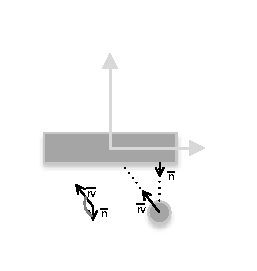
\includegraphics[scale = 1.5]{closing.pdf}
	\caption{Visualization of the closing feature. The gray half circle shows the angle whose weighted cosine is computed by the feature.} 
	\label{fig:closing}
\end{figure} 

The other relative features are computed by transforming their global counterparts to the coordinate system of the reference object. Equation \ref{eq:trans} shows this exemplary for the position:

\begin{equation}
	\vec{relPos} = T^{-1} \times \vec{gPos}
\label{eq:trans}
\end{equation}

where $T^{-1}$ is the transformation matrix computed from the reference objects orientation and global position as defined by equation \ref{eq:transMatrix}. $\vec{gPos}$ is the position vector of the second object in homogeneous coordinates. The same transformation is required when computing the change in an object's state using the old object's state as reference. 

The distance is calculated by computing the distances from all corners of one objects to all edges of the second object. 
The distance between the two objects corresponds to the closest of these corner-edge distances. In case of round objects, such as the actuator, the center is considered as a corner and the radius is subtracted from the computed distance.


\subsection{From target object state to action primitive \label{sec:gatePlanningReal}}

The overall process of computing a suitable action primitive that allows to push an object towards a given target configuration is quite similar to the one in the previous model that is explained in section \ref{sec:pairPlanningReal}. However, due to the differences in representation, the process is actually easier in this model. 
First of all, since the model works directly with the object states, the target representation does not need to be changed. A specified target object state can directly be used by the model. 
Furthermore, for each object group only one inverse model exist, which directly avoids the problems with multiple local inverse models mentioned in section \ref{sec:pairPlanningReal}. 

The preconditions are computed as already visualized in figure \ref{fig:GatePlanning}: \\
First the local difference vector\footnote{Local mean here that the difference vector is computed with respect to the current object's coordinate frame.} between the current object state and the target state is calculated.
Afterwards, the local inverse model responsible for the given object is queried for the preconditions given this difference vector. The actual computation of these preconditions is explained in section \ref{sec:invModelRealization}.

Once the preconditions have been computed, the same analysis as in the other model needs to be performed. These preconditions are in the form of the relative interaction features described above.
Unlike in the prediction case, the model needs to have knowledge about what some of the features represent. Specifically, the information about the local actuator position $\vec{p}_{cond}$ needs to be extracted from these preconditions. Afterwards, $\vec{p}_{cond}$ can be compared with the local actuator position $\vec{p}_{cur}$. $\vec{p}_{cur}$ is extracted from the current relative interaction features between the object and the actuator. 
If these two positions are too far apart\footnote{This implementation considers an euclidean distance of 0.1 as too far apart. This threshold has proven to be suitable in the environment presented in section \ref{sec:environment}.} a circling action is performed. Unfortunately, this needs to be provided by the user since the model has no information about the shape of the objects or what circling means. In this implementation, each object state, that needs to be defined by the user anyways, provides a method that computes an action that circles the actuator around the object in a fixed distance.
The algorithm used to compute the circling action is described in Appendix \ref{sec:circling}.

The model uses a circling action instead of directly moving towards the desired position, because the target position might be on another side of the object. When moving the actuator straight towards $\vec{p}_{cond}$ the object might be influenced in a negative way.

If the actuator is close but not close enough\footnote{This implementation considers a euclidean distance of < 0.01 as close enough.} the direction $\vec{d} = \vec{p}_{cond} - \vec{p}_{cur}$ can be used as action primitive.
However, regardless of how fine the \enquote{closeness} threshold is set, the object might still be in the way of this direction in some cases. In order to avoid, moving the object in an unintended way, the direction is only followed if the gate predicts that the next action will not influence the object. Otherwise, the same circling movement as described above is performed.

Once the actuator is close enough to $\vec{p}_{cond}$, the actual action primitive needs to be extracted from the preconditions. 
While the action primitives were directly included in the preconditions in the interaction state model, they are not included in the preconditions for this model. 
However, the relative interaction features include the relative velocity of the actuator. 
Since the action primitives control velocities in this scenario, the direction of this relative velocity can be used to construct an action primitive that points in the same direction. Afterwards, the action primitive needs to be transformed to the global coordinate frame, using the transformation matrix $T$ as explained above.

As mentioned in the interaction state model above (section \ref{sec:pairPlanningReal}), in case no precondition could be returned by the \gls{tiim}, exploration would be required. However since this was not a focus of this thesis only a random action in the general direction of the object is used which
can lead to the model getting stuck. Therefore, it is assumed that the inverse model as been trained sufficiently before a target configuration is to be reached.

\section{Used technologies \label{sec:technologies}}

\subsection{The Averaging Inverse Model \label{sec:invModelRealization}} 

The \acrfull{tiim} was suggested in the previous chapter in order to deal with the problems involved in computing the input from a given output. In this setting, the problem of extrapolation is the most important one since the models are supposed to reach any target instead of only ones that are reachable by performing a single action primitive.

This special inverse model is designed to learn typical preconditions that result in a certain change in the features. It is less important how strong the change is, but rather in what direction (positive or negative) a feature dimension changes. The idea is to compute the average preconditions for each feature dimension and each direction this dimension changes in. This assumes, that similar situations result in similar changes, for example if a block is pushed from the left it moves to the right.
 
These preconditions depend on the actual model. In case of the interaction state model, the combination of interaction state and action primitive is used while the gating model uses the relative interaction features. However, as described in sections \ref{sec:pairPlanningReal} and \ref{sec:gatePlanningReal}, this average can be used to derive an action primitive in both cases.

The implementation of this inverse model consists of two parts: 
\begin{itemize}
\item A \textit{network}
\item Its nodes (\textit{prototypes})
\end{itemize}

\textbf{Network:}

The network is the main part of the inverse model. It contains and manages the different prototypes. 
As explained in the sections for both models, the inverse model is trained on the preconditions and the difference vector. The difference vector $\vec{d}$ represents either the changes in an interaction or an object state depending on the used model.

For each actually changing feature dimension within $\vec{d}$ the network creates up to two prototypes. One for positive and one for negative changes within that dimension. That way a prototype represents changes in a given direction (positive or negative) of one specific feature dimension. 

In the example in figure \ref{fig:InverseModel} three different pushing interactions between the actuator and an object are seen. 
When the network is trained on these situations, three prototypes are created: One for the position change upwards and one for each rotation direction. 
Since all three situations result in an upward positional change, the corresponding prototype averages the preconditions of all three situations.
On the other hand, the two orientation prototypes will only be trained on one situation each.

The network is queried to provide preconditions that reduce a given difference vector. Ideally, preconditions that reduce the difference in all features at the same time would be returned. 
However, averaging the preconditions returned by different prototypes is prone to produce invalid preconditions. 
Furthermore, depending on the environment, it might not always be possible to reduce all features at the same time. 

In order to avoid invalid preconditions, the network uses a greedy strategy of reducing the feature dimension with the biggest difference\footnote{In order to avoid oscillations between different features and preconditions, the network remembers the selected feature until the sign in the difference flips or the feature difference $||f|| < \epsilon_{Index}$. Again this threshold depends on the expected change of features in the environment.}. Since the feature dimensions are not normalized, the biggest numerical value might not correlate to what humans regard as a big distance. 
However, this approach works quite well in practice, considering the inverse model does not have any knowledge about the feature's characteristics. 

Once the feature dimension with the biggest difference has been chosen, the corresponding prototype returns up to two possible preconditions as explained below.
The prototypes are asked to return two preconditions where possible in order to allow greater flexibility of the network: \\
The network tries to determine preconditions that reduce the difference in the biggest feature dimension while also setting up future movements in order to reduce the next biggest difference. Consider the example in figure \ref{fig:avgProblem} where two valid alternative preconditions are visualized: If the block should not only be rotated counterclockwise but also moved upwards, the position below the block is more favorable. This is because, in order to reduce the positional difference, the preconditions averaged over the situations visualized in figure \ref{fig:InverseModel} would be used. On the other hand, if the block should be moved to the right, the other situation should be preferred.

In order to do that the network queries the preconditions for the second biggest feature dimension as well. By comparing the (euclidean) norms between the four preconditions it is possible to determine which of the two preconditions for the first feature dimension is closer to the preconditions of the second feature dimension.  

In case both alternatives for the first feature are deemed equally good, the first preconditions are used since these correspond to a greater change in the desired feature dimension.

Unfortunately, this strategy, does not always avoid choosing the suboptimal preconditions. Since the preconditions for the second biggest feature dimension can only ever be evaluated based on the current situation, wrong choices might be made. Consider the same example as above, but the block is supposed to be turned by 180°. In that case, the local positional difference, the inverse model tries to reduce, will change its sign by turning the block around. This means that in order to move the block upwards in the global sense after turning it around, the block needs to be pushed downwards regarding its local coordinate system. In this case, the alternative above the block in figure \ref{fig:avgProblem} would have been the better choice.

If the network is queried before it has been trained sufficiently, there might not be a prototype for the feature dimension with the biggest difference. In that case the network tries to reduce the second biggest feature dimension and so forth. If no prototype can be found for the remaining differences, the network cannot return any preconditions which it indicates by returning a null value. 

\textbf{Prototype:}

Within a prototype, all collected preconditions are averaged by weighting each input by the magnitude of the change in the feature dimension in $\vec{d}$ that the input caused.
In the example in figure \ref{fig:InverseModel}, the middle scenario receives the biggest weight, since it changes the position more then the outer situations. 

While this average works great in the given example for the positional node, it does not work for all features as can be seen in figure \ref{fig:avgProblem}.

\begin{figure}
	\centering
	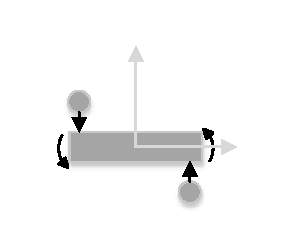
\includegraphics{avgProblem.pdf}
	\caption{Visualization of two alternative preconditions for a positive rotation of the block. The circles represent the actuator while the rectangle represents a block object. The gray arrows symbolize the local coordinate system of the block. Averaging these preconditions in the prototype would result in an invalid precondition.} 
	\label{fig:avgProblem}
\end{figure}

Consider the orientation prototype for positive rotations around the z-axis as shown in the figure. The magnitude of the change is identical in both situations, meaning that normally, the mean of both preconditions should be used as the average. In the given situation, this results in invalid preconditions, where the actuator would be supposed to be in the center of the object. That position is not only not reachable, but it also would not produce the desired change in orientation. 

In order to prevent this, multiple averages are computed in a prototype. Basically, the prototypes store a separate average for each combination of signs in the input data. This model uses three different sign possibilities: \textit{+}, \textit{-} and \textit{0}\footnote{The sign is considered 0 if the feature $||f|| < \epsilon_{Node}$. This threshold depends on the expected change of the features.}.
Going back to the example in figure \ref{fig:avgProblem}, assume that the following four input features are used: relative $x$ and $y$ position and relative $x$ and $y$ velocities of the actuator. All feature are represented in the object's coordinate frame. Table \ref{tab:signCombinations} shows the sign combinations that are experienced in the two given situations. 

\begin{table}
	\centering
	\begin{tabular}{|c|c|c|}
		\hline Feature & Combination 1 & Combination 2 \\ 
		\hline x position & \textit{+} & \textit{-} \\ 
		\hline y position & \textit{-} & \textit{+} \\ 
		\hline x velocity & \textit{0} & \textit{0} \\
		\hline y velocity & \textit{+} & \textit{-} \\ 
		\hline 
	\end{tabular} 
	\caption{The sign combinations of preconditions in the example in figure \ref{fig:avgProblem}.}
	\label{tab:signCombinations}
\end{table}

In this case, averages for both possible combinations are updated in the prototype. More specifically, for each different combination the prototype stores the sum of the contributions, the sum of all inputs as well as the number of times this combination was experienced. 

Unfortunately, noisy data will lead to the creation of multiple combinations that are basically equivalent. For example it might be, that due to some motor or sensor noise, a small $x$ velocity $>\epsilon_{Node}$ was detected in one of the two situations. In that case a third combination with an x velocity sign different from \textit{0} is created as well. As long as this velocity is very small, this combination would still be valid. In the worst case noise can create invalid combinations. An example would be if the sensors pick up a change in the object's orientation although the actuator moved away from the object. Since the model cannot know what is a valid training example and what is invalid noise, all combinations are created equally.

When the prototype is asked to return the averaged preconditions, it tries to find up to two valid combinations for the network. These two combinations would ideally represent two valid but different alternatives, as in the example above. 
In order to create these averages, the following steps are performed:
\begin{enumerate}
\item Merge equivalent (valid) combinations.
\item Select up to two merged combinations with the highest contribution.
\item Compute averages from these two combinations.
\end{enumerate}

\textbf{1) Merging:}

The prototypes try to merge equivalent combinations. This is done, by making a special assumption about features with a \textit{0} sign: If an input feature has been experienced to be close to \textit{0} for a given prototype, then it should be possible to average over all occurrences of this feature. 
In this sense, combinations are considered equivalent and are merged, if they do not have any opposing signs at any of their input features.
Table \ref{tab:signCombinations2} summarizes the sign combinations experienced from the three scenarios in the first example, presented in figure \ref{fig:InverseModel}.
Since a \textit{0} does not oppose either a \textit{+} or a \textit{-}, all three combinations can be merged together.
Depending on the used features and the amount of noise in the data, special care needs to be given when merging combinations. In the example above, the resulting combination should ideally represent a x position close to 0 since that would result in the biggest positional change. In case the weights of either combination 1 or combination 3 is significantly bigger than the other, the average over all three situations would result in an x position different from 0.
In order to further avoid such undesired effects, the merging process can be made more strict by only combining combinations that are similar even in their \textit{0} signs.
This implementation allows only one feature dimension to differ after the opposing sign check in order to better preserve \textit{0} sign feature dimensions.

\begin{table}
	\centering
	\begin{tabular}{|c|c|c|c|}
		\hline Feature & Combination 1 & Combination 2 & Combination 3 \\ 
		\hline x position & \textit{+} & \textit{0} & \textit{-} \\ 
		\hline y position & \textit{-} & \textit{-} & \textit{-} \\ 
		\hline x velocity & \textit{0} & \textit{0} & \textit{0} \\
		\hline y velocity & \textit{+} & \textit{+} & \textit{+} \\ 
		\hline 
	\end{tabular} 
	\caption{The three sign combinations for the example in figure \ref{fig:InverseModel} where the block is pushed at three different positions from below.}
	\label{tab:signCombinations2}
\end{table}

The actual merging process is described in algorithm \ref{alg:combinationMerging}. The sign combination of a given precondition is used as \textit{key} in order to reference the corresponding weights, the sum of preconditions and the number of occurrences of that sign combination. 
In order to avoid merging invalid combinations, the combinations are first filtered. This model assumes, that valid combinations are experienced more often than invalid ones that are results from noise. 
Especially, since small noise can also be filtered out by only considering feature changes above a certain threshold when training the prototypes. That way, all combinations that have been experienced less often then the average number of experiences over all combinations are filtered out. 
The resulting combinations are checked for their equivalence by iteratively comparing the combination with the most \textit{0}s to all other combinations until all have been processed.

\begin{algorithm}[H]
\begin{algorithmic}[1]
	\Require{List of combinations L}
	\Require{Hashmap of combination weights W}
	\Require{Hashmap of combination input sums I}
	\Require{Hashmap of combination occurence numbers N}
	
	\Ensure{Hashmap of merged combination weights W$^*$}
	\Ensure{Hashmap of merged combination input sums I$^*$}
	\Ensure{Hashmap of merged combination occurrence numbers N$^*$}
	\Statex
	\Let{usefulKeys}{filterInvalidCombinations(L, N)}
	\Let{sortedKeys}{sortByNumZeros(usefulKeys)}
	\While{sortedKeys not empty}
		\Let{currentKey}{sortedKeys[0]}
		\Let{tmpWeight}{0}
		\Let{tmpSum}{0}
		\Let{tmpNumber}{0}
		\ForAll{key in sortedKeys}
			\If{isEquivalent(currentKey, key)}
				\Let{tmpWeight}{tmpWeight + W[key]}
				\Let{tmpSum}{tmpSum + I[key]}
				\Let{tmpNumber}{tmpNumber + N[key]}
				\State remove key from sortedKeys
			\EndIf
		\EndFor
		\Let{newKey}{recomputeCombination(tmpSum, tmpWeight)}
		\Let{W$^*$[newKey]}{tmpWeight}
		\Let{I$^*$[newKey]}{tmpSum}
		\Let{N$^*$[newKey]}{tmpNumber}
	\EndWhile
\end{algorithmic}
\caption{Description of the merging process for combinations within a node.}
\label{alg:combinationMerging}
\end{algorithm}

After equivalent combinations have been merged, the resulting input features might represent a new sign combination. This combination is computed and used as the new key for storing the resulting values. 


\textbf{2) Selecting combinations with the highest contribution:}

If only one combination remained after the merging process, the preconditions from that combination are returned. 
Otherwise, the prototype sorts the resulting combinations based on their average contribution. This can easily be computed by dividing the total weight by the number of experiences for each combination.
In that case the best two combinations are considered if their average contribution is not too far apart\footnote{In this implementation this means, that the second highest average contribution is not less then half of the highest average contribution.}. Otherwise, only the best combination is used as if no alternative exist.

\textbf{3) Compute preconditions:}

From the two combinations with the biggest contribution, two preconditions are computed as described in algorithm \ref{alg:averaging}.

\begin{algorithm}[h]
\begin{algorithmic}[1]
	\Require{$\vec{pre}_1$ Input sum of the first combination}
	\Require{$\vec{pre}_2$ Precondition sum of the second combination}
	\Require{$w_1$ Total weight for the first combination}
	\Require{$w_2$ Total weight for the second combination}
	\Require{$\vec{comp}_1$ Vector containing feature signs for the first combination}
	\Require{$\vec{comp}_2$ Vector containing feature signs for the second combination}
	\Ensure{$\vec{average}_1$}
	\Ensure{$\vec{average}_2$}
	\Statex
	\Let{size}{len($\vec{comp}_1$)}
	\For{i = 1..size}
		\Let{c$_{1i}$}{$\vec{comp}_1$[i]}
		\Let{c$_{2i}$}{$\vec{comp}_2$[i]}
		\If{c$_{1i}$ == c$_{2i}$}
			\Let{$\vec{average}_1$[i]}{$\frac{pre_{1i} + pre_{2i}}{w_1+w_2}$}
			\Let{$\vec{average}_2$[i]}{$\vec{average}_1$[i]}
		\Else
			\Let{$\vec{average}_1$[i]}{$\frac{pre_{1i}}{w_1}$}
			\Let{$\vec{average}_2$[i]}{$\frac{pre_{2i}}{w_2}$ }
		\EndIf
	\EndFor
\end{algorithmic}
\caption{Description of the averaging process within the nodes if at least two combinations are present.}
\label{alg:averaging}
\end{algorithm}

The signs of both combinations are compared and the feature dimensions in the preconditions of both combinations are averaged if their signs are identical.
The feature dimensions are considered separately otherwise.

Using these two components of the network and its prototypes, it is possible to abstract from the actual quantities in feature changes during training and instead focus in the direction. For the purpose of incrementally reaching target configurations this direction is sufficient in combination with the circling strategies explained in sections \ref{sec:pairPlanningReal} and \ref{sec:gatePlanningReal}.


\subsection{Adapted Instantaneous Topological Map \label{sec:ITM}}

The underlying regression and classification model that is used throughout this thesis is an adaptation of the \acrfull{itm} and is therefore called \acrfull{aitm} throughout this thesis.
The \gls{itm} \cite{itm} itself is an adaptation of the \gls{gng} \cite{gng} algorithm to create topological maps. Instead of \glspl{gng} global update rules for inserting new nodes in the map, the \gls{itm} uses local update rules in order to be better suited for correlated inputs. 
In order to be applicable to classification and regression, the \gls{itm} was further extended by an output function using the idea of \gls{llm} \cite{LLM}. In order to extend a topological map with an output function, each node represent the corresponding output vector $\vec{w}^i_{out}$ along its input vector $\vec{w}^i_{in}$. The \gls{llm} extends each node further with a local linear mapping $A^i$. This matrix is used to improve the function approximation within each Voronoi cell. With this, the output of each node given an input vector $\vec{x}$ is computed by equation \ref{eq:llmOut}:

\begin{equation}
\vec{y}^i(\vec{x}) = \vec{w}^i_{out} + A^i \cdot (\vec{x}-\vec{w}^i_{in})
\label{eq:llmOut}
\end{equation}

The output function for the network can be computed in multiple ways. The simplest method is to use the output of the winning node, i.e. the output of the node whose input vector $\vec{w}^i_{in}$ is closest to the given input $\vec{x}$. In order to reduce the effect of the metric problem when finding the closest node, the outputs of multiple nodes can also be mixed together. % using a softmax weighting similar to the idea in \cite{NIPS2010_3895}. 
The evaluations in this thesis interpolate the output functions of the two closest nodes:

\begin{equation}
\vec{y}_{net}(\vec{x}) =  \frac{1}{k_n+k_s} \cdot \left[ k_n \cdot \left(\vec{w}^n_{out} + A^n \cdot \left(\vec{x}-\vec{w}^n_{in}\right)\right) + k_s \cdot  \left(\vec{w}^s_{out} + A^s \cdot \left(\vec{x}-\vec{w}^s_{in}\right)\right)\right]
\end{equation}

where $k_n$ and $k_s$ are the weights or importance for the nearest and the second node respectively. These weights are computed as follows:

\begin{equation}
\begin{split}
k_n = \exp\left(\frac{||\vec{x}-\vec{w}^n_{in}||}{\sigma^2}\right) \\
k_s = \exp\left(\frac{||\vec{x}-\vec{w}^s_{in}||}{\sigma^2}\right) 
\end{split}
\end{equation}

$\sigma$ determines the influence radius of each node, just like in radial basis networks \cite{rbf}.
The nearest node $n$ and the second closest node $s$ are determined by comparing the input vectors of all nodes in $W$ with the given input vector $\vec{x}$:

\begin{equation}
\begin{split}
	nearest: n = \argmin_{c \in W} ||(\vec{x} - \vec{w}^c_{in})|| \\
	second: s = \argmin_{c \in W\backslash\{n\}} ||(\vec{x} - \vec{w}^c_{in})||
\end{split}
\label{eq:itmNearest}
\end{equation}

During training, the network receives an input-output pair and updates its nodes. First, the two closest nodes $nearest$ and $second$ are computed as stated in equation \ref{eq:itmNearest}. Afterwards, only the node $nearest$ is adapted in accordance to the update rules of the \gls{llm}:

\begin{equation}
\begin{split}
\Delta \vec{w}^n_{in} = \eta_{in} \cdot (\vec{x}^\alpha - \vec{w}^n_{in}) \\
\Delta \vec{w}^n_{out} = \eta_{out} \cdot (\vec{y}^\alpha - \vec{y}^n(\vec{x}^\alpha)) + A^n \cdot \delta \vec{w}^n_{in} \\
\Delta A^n = \eta_A \cdot (\vec{y}^\alpha - \vec{y}^n(\vec{x}^\alpha)) \frac{(\vec{x}^\alpha - \vec{w}^n_{in})^t}{||\vec{x}^\alpha - \vec{w}^n_{in}||^2}
\end{split}
\end{equation}

The initial matrix $A$ is a zero matrix with proper dimensions\footnote{Usually one initializes the matrix $A$ at random or with prior knowledge. However, in this thesis a zero matrix is used in order to avoid using invalid linear interpolations while the matrix has not been adapted to the data.}. 
The learning rates $\eta_{in}, \eta_{out}$ and $\eta_A$ are meta parameters that need to be determined. In case $\eta_A$ is set to 0, no linear approximation is learned for each Voronoi cell. This means, that each cell has only the constant output of $\vec{w}^n_{out}$. This thesis uses a $\eta_{A} = 0$ because the differences between $\vec{x}^\alpha$ and  $\vec{w}^n_{in}$ are often very small, which results in numeric instabilities when updating the matrix $A$. 

After the winning node has been updated, the classical \gls{itm} algorithm uses local relations between the new input, the winning node and the second node in order to determine if a new node should be inserted or if some node should be deleted. As long as there are no big jumps in consecutive training samples, this approach works quite well. However, when resetting the environment between consecutive training runs, larger gabs can arise. Furthermore, this network has already been extended by an output function which can now also be used during training. This \gls{aitm} inserts new nodes into the network based on the difference between the current output of the network and the target output:

\begin{equation}
||\vec{y}^{net}(\vec{x}^\alpha)-\vec{y}^\alpha|| > \epsilon_{ITM}
\label{eq:newNode}
\end{equation}

If the output varies too much, a new node at the position of $\vec{x}^\alpha$ and output $\vec{y}^\alpha$ is created unless its distance to the winning node is too small

\begin{equation}
||\vec{x}^\alpha - \vec{w}^n_{in}|| \le \epsilon_{max}
\end{equation}

$\epsilon_{max}$ represents the maximum distance nodes should be apart and needs to be chosen to represent the order of magnitude of the norm of the input vectors.
If the new input is too close to the winning node although the output was not similar enough, the output of the winning node is adapted with:

\begin{equation}
\Delta\vec{w}^n_{out} = 0.5 \cdot (\vec{y}^\alpha - \vec{w}^n_{out})
\end{equation}

This ensures, that noisy data does not lead to the creation of multiple nodes with similar input vectors. 

The threshold $\epsilon_{ITM} = 10^d$ is dynamically computed, based on the order of magnitude $d$ of the target output norm:

\begin{equation}
d = \begin{cases}
\lfloor\log_{10}(||\vec{y}^\alpha||)\rfloor & \text{, if $||\vec{y}^\alpha|| > 0$} \\
\lfloor\log_{10}(||\vec{y}^\alpha||)\rfloor-1 & \text{, if $log_{10}(||\vec{y}^\alpha||) = 0$} \\
-k & \text{, otherwise}
\end{cases}
\end{equation}

When the output has a norm of $0$ a fixed threshold $10^k$ is chosen. Ideally $k$ should represent the average order of magnitude of the input. This average can be computed incrementally from the non-zero output norms\footnote{In this prototypes a fixed $k=3$ is chosen instead.}. The benefit of such a dynamic threshold is that it automatically adapts to different use cases. For example, when the \gls{aitm} is used for classification, the output values will be class labels in the form of positive natural numbers. In this case $d$ equals $-1$ which results in a threshold of 0.1 which allows to distinguish conflicting class labels\footnote{The special treatment for this case is done in order to conform to the $>$ in equation \ref{eq:newNode}, the case can be omitted if $>=$ is used instead, however testing for the equal case is less robust in the regression case.}.
In regression tasks however, the output values will be real numbers. It is obvious that different thresholds are required for both types of use case. The \gls{aitm} assumes that the orders of magnitude of the output within one use case are generally rather similar and can be used as an approximation of the desired accuracy.

With every update the two winning nodes are connected as neighbors. Node deletions are performed just as in the traditional \gls{itm}: Second winners are removed if they are too far away from the winning node, i.e.:
\begin{equation}
||\vec{w}^n_{in} - \vec{w}^s_{in}|| > \epsilon_{max}
\end{equation}

Furthermore, isolated nodes will be deleted. A node is considered isolated if it does not have any neighbors left. Neighbor connections are removed if the second winner in an update can replace a previous neighbor:

\begin{equation}
\forall c \in N(n): \text{If~} (\vec{w}^n_{in}-\vec{w}^s_{in}) \cdot (\vec{w}^c_{in}-\vec{w}^s_{in}) < 0 \text{~remove connection (n,c)}
\end{equation}

$N$ denotes the set of neighbors of the winning node $n$.

All norms that are used here are euclidean norms which might not be ideal depending on the used features. However, since the models should not be provided with additional knowledge about the features, this common choice was made.

